% $Header: /Users/joseph/Documents/LaTeX/beamer/solutions/conference-talks/conference-ornate-20min.en.tex,v 90e850259b8b 2007/01/28 20:48:30 tantau $

\documentclass[10pt,serif, professionalfont]{beamer}

% This file is a solution template for:

% - Talk at a conference/colloquium.
% - Talk length is about 20min.
% - Style is ornate.



% Copyright 2004 by Till Tantau <tantau@users.sourceforge.net>.
%
% In principle, this file can be redistributed and/or modified under
% the terms of the GNU Public License, version 2.
%
% However, this file is supposed to be a template to be modified
% for your own needs. For this reason, if you use this file as a
% template and not specifically distribute it as part of a another
% package/program, I grant the extra permission to freely copy and
% modify this file as you see fit and even to delete this copyright
% notice. 


\mode<presentation>
{
  %\usetheme{Singapore}
  %\usetheme{Goettingen}
  \usetheme{Pittsburgh}
  % or ...

  %\setbeamercovered{transparent}
  % or whatever (possibly just delete it)

  \usecolortheme{dove}
  %\usecolortheme{seagull}
  %\setbeamertemplate{blocks}[rounded][shadow=false]
  %\setbeamertemplate{background canvas}[vertical shading][bottom=white,top=structure.fg!25]
  %\setbeamercolor{block body}{bg=normal text.bg!90!black}
  %\setbeamertemplate{sidebar canvas left}[horizontal shading][left=white!40!black,right=black]
}


\usepackage[english]{babel}
% or whatever

\usepackage[utf8]{inputenc}
% or whatever

%\usepackage{times}
\usepackage[T1]{fontenc}
% Or whatever. Note that the encoding and the font should match. If T1
% does not look nice, try deleting the line with the fontenc.

\usepackage{concrete}

\usepackage{graphicx}
\usepackage{float}
\usepackage{amsmath}
\usepackage{amsthm}
\usepackage{amssymb}
\usepackage{caption}
\usepackage{bbold}


\title%[Short Paper Title] % (optional, use only with long paper titles)
{Patterns in Riordan arrays}

%\subtitle {Include Only If Paper Has a Subtitle}

\author[Merlini, Nocentini] % (optional, use only with lots of authors)
{Donatella Merlini\inst{1} \and Massimo Nocentini}
% - Give the names in the same order as the appear in the paper.
% - Use the \inst{?} command only if the authors have different
%   affiliation.

\institute[Universities of Somewhere and Elsewhere] % (optional, but mostly needed)
{
  \inst{1}%
  Dipartimento di Statistica, Informatica, Applicazioni\\
  Universit\`a di Firenze, Italy
  %\and
  %\inst{2}%
  %Department of Theoretical Philosophy\\
  %University of Elsewhere
    \begin{center}
        
\includegraphics[width=3cm]{logo/unifi} \\ \medskip
    \end{center}
  }
% - Use the \inst command only if there are several affiliations.
% - Keep it simple, no one is interested in your street address.


\date[RART2015] % (optional, should be abbreviation of conference name)
{RART, 2015}
% - Either use conference name or its abbreviation.
% - Not really informative to the audience, more for people (including
%   yourself) who are reading the slides online

\subject{Theoretical Computer Science}
% This is only inserted into the PDF information catalog. Can be left
% out. 



% If you have a file called "university-logo-filename.xxx", where xxx
% is a graphic format that can be processed by latex or pdflatex,
% resp., then you can add a logo as follows:

\pgfdeclareimage[height=0.5cm]{university-logo}{logo/unifi}
\logo{\pgfuseimage{university-logo}}



% Delete this, if you do not want the table of contents to pop up at
% the beginning of each subsection:
\AtBeginSubsection[]
{
  \begin{frame}<beamer>{Outline}
    \tableofcontents[currentsection,currentsubsection]
  \end{frame}
}


% If you wish to uncover everything in a step-wise fashion, uncomment
% the following command: 

%\beamerdefaultoverlayspecification{<+->}


\begin{document}


\begin{frame}
  \titlepage
\end{frame}

\begin{frame}{Outline}
  \tableofcontents
  % You might wish to add the option [pausesections]
\end{frame}


% Structuring a talk is a difficult task and the following structure
% may not be suitable. Here are some rules that apply for this
% solution: 

% - Exactly two or three sections (other than the summary).
% - At *most* three subsections per section.
% - Talk about 30s to 2min per frame. So there should be between about
%   15 and 30 frames, all told.

% - A conference audience is likely to know very little of what you
%   are going to talk about. So *simplify*!
% - In a 20min talk, getting the main ideas across is hard
%   enough. Leave out details, even if it means being less precise than
%   you think necessary.
% - If you omit details that are vital to the proof/implementation,
%   just say so once. Everybody will be happy with that.

\section{Motivation}

\subsection{Some definitions}

\begin{frame}{Riordan arrays}
    We consider  Riordan arrays of the form $\mathcal{R}\left( d(t), h(t)\right)$
    where:
    \begin{displaymath}
        d_{nk}\in\mathcal{R} \leftrightarrow d_{nk} = \big[t^{n}\big]d(t)\,h(t)^{k}
    \end{displaymath}

    Let $\mathcal{R}$ be a Riordan array and $p$ be a prime.
    
    \begin{block}{$\mathcal{R}_{\equiv_{p}}$}
        Define $\mathcal{R}_{\equiv_{p}}$
        as the \emph{congruent of} $\mathcal{R}$, modulo $p$, such that:
        \begin{displaymath}
            d_{nk}\in\mathcal{R} \leftrightarrow a \in\mathcal{R}_{\equiv_{p}}
            \quad \text{where} \quad d_{nk}\equiv_{p} a
        \end{displaymath}
    \end{block}

    \begin{block}{$\mathcal{R}^{(\alpha)}$}
        Define $\mathcal{R}^{(\alpha)}$
        as the \emph{principal $\alpha$-cluster of} $\mathcal{R}$, such that:
        \begin{displaymath}
            d_{nk}\in\mathcal{R}^{(\alpha)}\rightarrow d_{nk}\in\mathcal{R}
            \quad \text{where}\quad n\in\lbrace0,\ldots,p^{\alpha}-1\rbrace
        \end{displaymath}
    \end{block}
    

\end{frame}

\begin{frame}{Riordan arrays}
    $\mathcal{P}$ascal and $\mathcal{F}$ibonacci arrays, respectively:
    \begin{displaymath}
            \mathcal{P}\left(\frac{1}{1-t},\frac{t}{1-t}\right) \quad\quad 
                \mathcal{F}\left(\frac{1}{1-t-t^2}, \frac{1-\sqrt{1-4t}}{2} \right)
    \end{displaymath}

    $\mathcal{D}$elannoy and $\mathcal{C}$atalan arrays, respectively:
    \begin{displaymath}
        \mathcal{D}\left(\frac{1}{1-t},\frac{t(1+t)}{1-t}\right) \quad\quad
            \mathcal{C}\left(\frac{1-\sqrt{1-4t}}{2t}, \frac{1-\sqrt{1-4t}}{2}\right)
    \end{displaymath}

    finally, $\mathcal{M}$otzkin array:
    \begin{displaymath}
        \mathcal{M}\left(\frac{1-t-\sqrt{1-2t-3t^2}}{2t^2}, \frac{1-t-\sqrt{1-2t-3t^2}}{2t}\right)
    \end{displaymath}
\end{frame}

\subsection{Previous Work}

\begin{frame}{Fine, Sved et al.}

    \begin{block}{Fine in \ldots exposes \emph{Lucas theorem}}
        Let $p$ be a prime, $a=(a_{0},\ldots,a_{k})_{p}$ and $b=(b_{0},\ldots,b_{k})_{p}$, for some $k\in\mathbb{N}$:
        \begin{displaymath}
            {{a}\choose{b}} \equiv_{p} {{a_{0}}\choose{b_{0}}}{{a_{1}}\choose{b_{1}}}
                \ldots{{a_{k}}\choose{b_{k}}}
        \end{displaymath}
    \end{block}
    \pause
    \begin{block}{Sved in \cite{Sved1998} introduces:}
        \begin{itemize}
            \item {\normalsize a language to talk about triangles modulo some prime $p$}\\
                \footnotesize{\emph{principal cell}, \emph{principal $\alpha$-cluster}, \emph{zero-holes of order $\alpha$}}
            \item {\normalsize a graphic interpretation of \emph{Lucas theorem} }\\
                \footnotesize{each ${{a_i}\choose{b_i}}$ locates ${{a}\choose{b}}$ within a \emph{nest of triangles}}
            \item {\normalsize an application of \emph{Lucas theorem} to Stirling triangle}\\
                \footnotesize{via a \emph{mapping} over the numbers of the second kind}
            \item {\normalsize higher powers of primes}\\
                \footnotesize{emphasizing coefficient $d_{nk}$ such that 
                    $p^{\alpha}\mid d_{nk}$ while $p^{\alpha+1}\nmid d_{nk}$}
        \end{itemize}
    \end{block}
\end{frame}

\begin{frame}{Fine, Sved et al.}
    \begin{block}{Wolfram in \ldots shows:}
        \begin{itemize}
            \item {\normalsize \emph{fractal dimensionality} of self-similar patterns in $\mathcal{P}_{\equiv_{2}}$}\\
                \footnotesize{solving recurrence $T(\frac{i}{2})=3\,T(i)$ yield $T(i)\approx i^{-\log_{2}{3}}$}
            \item {\normalsize $N(n)=\sum_{k=0}^{n}{\mathbb{1}_{{{n}\choose{k}}\equiv_{2}1}}$ is a very irregular function }\\
                \footnotesize{also $N(n)=2^{\phi_{1}(n)}$, where $ \phi_{1}((n_{0},n_{1},\ldots,n_{m})_{2})=
                    \sum_{j=0}^{m}{\mathbb{1}_{n_{j}=1} }$}
        \end{itemize}
    \end{block}
    \pause
    \begin{block}{Broomhead in \ldots shows:}
        \begin{itemize}
            \item {\normalsize $N(n)=\sum_{k=0}^{n}{\mathbb{1}_{p\nmid{{n}\choose{k}}}}$ has a closed form }\\
                \footnotesize{namely $N((n_{0},n_{1},\ldots,n_{m})_{2})=(n_{0}+1)(n_{1}+1)\cdots(n_{m}+1)$}
        \end{itemize}
    \end{block}
    \pause
    \begin{block}{McLean in \ldots generalizes:}
        Broomhead and Sved work over higher power of a prime $p$:
        \begin{itemize}
            \item defines \emph{$p$-index of $a$} as {$\nu_{p}\lbrace a\rbrace =t \leftrightarrow p^{t}\mid a \wedge p^{t+1}\nmid a$}
            \item proves {$\nu_{p}\lbrace {{n}\choose{k}}\rbrace $} equals the \emph{number of carries} in $n-_{p}k$
        \end{itemize}
    \end{block}
\end{frame}

\section{Some arrays and their congruents}

\subsection{Colouring for some primes}

%\subsection{Pascal}

\begin{frame}{$\mathcal{P}_{\equiv_{2}}$ where 
    $\textcolor{blue}{[0]_{2}},\textcolor{orange}{[1]_{2}}$}

    

\begin{figure}[p]
    
    \hspace{-1.5cm}
    \noindent\makebox[\textwidth]{
        \centering
        %\includegraphics[width=0.8\textwidth]{../../sympy/catalan/coloured.pdf}

        % using *angle* property to rotate it is difficult to properly align it
        % in order to have a "real" matrix representation.
        \includegraphics[width=20cm, height=20cm, keepaspectratio=true]{../sympy/pascal/pascal-standard-ignore-negatives-centered-colouring-127-rows-mod2-partitioning-triangle.pdf}
    }

    % this 'particular' line is necessary to use `displaymath' environment
    % into the caption environment, togheter with the inclusion of 
    % `caption' package. See here for more explanation:
    % http://stackoverflow.com/questions/2716227/adding-an-equation-or-formula-to-a-figure-caption-in-latex
    \captionsetup{singlelinecheck=off}
    \caption[$\mathcal{P}_{\equiv_{2}}$]{
        $\mathcal{P}_{\equiv_{2}}$
        \iffalse
        Pascal triangle, formally: 
        \begin{displaymath}
            \mathcal{P}=\left(\frac{1}{1-t}, \frac{t}{1-t}\right)
        \end{displaymath} % \newline % new line no more necessary
        standard, ignore negatives, centered colouring, 127 rows, mod2 partitioning
        \fi
        }

    \label{fig:pascal-standard-ignore-negatives-centered-colouring-127-rows-mod2-partitioning-triangle}

\end{figure}

\end{frame}

\begin{frame}{$\mathcal{P}_{\equiv_{3}}$ where 
    $\textcolor{blue}{[0]_{3}},\textcolor{orange}{[1]_{3}},\textcolor{red}{[2]_{3}}$}

    \input{../sympy/pascal/pascal-standard-ignore-negatives-centered-colouring-127-rows-mod3-partitioning-include-figure}
\end{frame}
\begin{frame}{$\mathcal{P}_{\stackrel{\circ}{\equiv_{3}}}$ where 
    $\textcolor{blue}{[0]_{3}},\textcolor{orange}{\lbrace [1],[2] \rbrace_{3}}$}

    
\begin{figure}[H]

    \noindent\makebox[\textwidth]{
        \centering
        %\includegraphics[width=0.8\textwidth]{../../sympy/catalan/coloured.pdf}

        % using *angle* property to rotate it is difficult to properly align it
        % in order to have a "real" matrix representation.
        \includegraphics[width=20cm, height=20cm, keepaspectratio=true]{../sympy/pascal/pascal-standard-ignore-negatives-centered-colouring-127-rows-multiples-of-3-partitioning-triangle.pdf}
    }

    % this 'particular' line is necessary to use `displaymath' environment
    % into the caption environment, togheter with the inclusion of 
    % `caption' package. See here for more explanation:
    % http://stackoverflow.com/questions/2716227/adding-an-equation-or-formula-to-a-figure-caption-in-latex
    \captionsetup{singlelinecheck=off}
    \caption[$\mathcal{P}_{\stackrel{\circ}{\equiv_{3}}}$]{ $\mathcal{P}_{\stackrel{\circ}{\equiv_{3}}}$ }

    \label{fig:pascal-standard-ignore-negatives-centered-colouring-127-rows-multiples-of-3-partitioning-triangle}

\end{figure}

\end{frame}
\begin{frame}{$\mathcal{P}_{\stackrel{\circ}{\equiv_{5}}}$ where 
    $\textcolor{blue}{[0]_{5}},\textcolor{orange}{\lbrace [1],[2],[3],[4] \rbrace_{5}}$}

    
\begin{figure}[H]

    \noindent\makebox[\textwidth]{
        \centering
        %\includegraphics[width=0.8\textwidth]{../../sympy/catalan/coloured.pdf}

        % using *angle* property to rotate it is difficult to properly align it
        % in order to have a "real" matrix representation.
        \includegraphics[width=20cm, height=20cm, keepaspectratio=true]{../sympy/pascal/pascal-standard-ignore-negatives-centered-colouring-127-rows-multiples-of-5-partitioning-triangle.pdf}
    }

    % this 'particular' line is necessary to use `displaymath' environment
    % into the caption environment, togheter with the inclusion of 
    % `caption' package. See here for more explanation:
    % http://stackoverflow.com/questions/2716227/adding-an-equation-or-formula-to-a-figure-caption-in-latex
    \captionsetup{singlelinecheck=off}
    \caption[$\mathcal{P}_{\stackrel{\circ}{\equiv_{5}}}$]{ $\mathcal{P}_{\stackrel{\circ}{\equiv_{5}}}$ }

    \label{fig:pascal-standard-ignore-negatives-centered-colouring-127-rows-multiples-of-5-partitioning-triangle}

\end{figure}

\end{frame}
\begin{frame}{$\mathcal{P}_{\stackrel{\circ}{\equiv_{7}}}$ where 
    $\textcolor{blue}{[0]_{7}},\textcolor{orange}{\lbrace [1],[2],[3],[4],[5],[6] \rbrace_{7}}$}

    
\begin{figure}[H]

    \vfill

    \hspace{-1.5cm}
    \noindent\makebox[\textwidth]{
        \centering
        %\includegraphics[width=0.8\textwidth]{../../sympy/catalan/coloured.pdf}

        % using *angle* property to rotate it is difficult to properly align it
        % in order to have a "real" matrix representation.
        \includegraphics[width=20cm, height=20cm, keepaspectratio=true]{../sympy/pascal/pascal-standard-ignore-negatives-centered-colouring-127-rows-multiples-of-7-partitioning-triangle.pdf}
    }

    % this 'particular' line is necessary to use `displaymath' environment
    % into the caption environment, togheter with the inclusion of 
    % `caption' package. See here for more explanation:
    % http://stackoverflow.com/questions/2716227/adding-an-equation-or-formula-to-a-figure-caption-in-latex
    \captionsetup{singlelinecheck=off}
    \caption[$\mathcal{P}_{\stackrel{\circ}{\equiv_{7}}}$]{ $\mathcal{P}_{\stackrel{\circ}{\equiv_{7}}}$ }

    \label{fig:pascal-standard-ignore-negatives-centered-colouring-127-rows-multiples-of-7-partitioning-triangle}

\end{figure}

\end{frame}

%\subsection{Fibonacci}

\begin{frame}{$\mathcal{F}_{\equiv_{2}}$ where 
    $\textcolor{blue}{[0]_{2}},\textcolor{orange}{[1]_{2}}$}

    
\begin{figure}[H]

    \noindent\makebox[\textwidth]{
        \centering
        %\includegraphics[width=0.8\textwidth]{../../sympy/catalan/coloured.pdf}

        % using *angle* property to rotate it is difficult to properly align it
        % in order to have a "real" matrix representation.
        \includegraphics[width=20cm, height=20cm, keepaspectratio=true]{../sympy/fibonacci/fibonacci-standard-handle-negatives-centered-colouring-127-rows-mod2-partitioning-triangle.pdf}
    }

    % this 'particular' line is necessary to use `displaymath' environment
    % into the caption environment, togheter with the inclusion of 
    % `caption' package. See here for more explanation:
    % http://stackoverflow.com/questions/2716227/adding-an-equation-or-formula-to-a-figure-caption-in-latex
    \captionsetup{singlelinecheck=off}
    \caption[$\mathcal{F}_{\stackrel{\circ}{\equiv_{2}}}$]{ $\mathcal{F}_{\stackrel{\circ}{\equiv_{2}}}$ }

    \label{fig:fibonacci-standard-handle-negatives-centered-colouring-127-rows-mod2-partitioning-triangle}

\end{figure}

\end{frame}
%\begin{frame}{$\mathcal{F}_{\equiv_{3}}$ where 
    %$\textcolor{blue}{[0]_{3}},\textcolor{orange}{[1]_{3}},\textcolor{red}{[2]_{3}}$}

    %\input{../sympy/fibonacci/fibonacci-standard-ignore-negatives-centered-colouring-127-rows-mod3-partitioning-include-figure}
%\end{frame}
\begin{frame}{$\mathcal{F}_{\stackrel{\circ}{\equiv_{3}}}$ where 
    $\textcolor{blue}{[0]_{3}},\textcolor{orange}{\lbrace [1],[2] \rbrace_{3}}$}

    
\begin{figure}[H]

    \hspace{1cm}
    \noindent\makebox[\textwidth]{
        \centering
        %\includegraphics[width=0.8\textwidth]{../../sympy/catalan/coloured.pdf}

        % using *angle* property to rotate it is difficult to properly align it
        % in order to have a "real" matrix representation.
        \includegraphics[width=15cm, height=15cm, keepaspectratio=true]{../sympy/fibonacci/fibonacci-standard-handle-negatives-centered-colouring-127-rows-multiples-of-3-partitioning-triangle.pdf}
    }

    % this 'particular' line is necessary to use `displaymath' environment
    % into the caption environment, togheter with the inclusion of 
    % `caption' package. See here for more explanation:
    % http://stackoverflow.com/questions/2716227/adding-an-equation-or-formula-to-a-figure-caption-in-latex
    \captionsetup{singlelinecheck=off}
    \caption[$\mathcal{F}_{\stackrel{\circ}{\equiv_{3}}}$]{ $\mathcal{F}_{\stackrel{\circ}{\equiv_{3}}}$ }

    \label{fig:fibonacci-standard-handle-negatives-centered-colouring-127-rows-multiples-of-3-partitioning-triangle}

\end{figure}

\end{frame}
\begin{frame}{$\mathcal{F}_{\stackrel{\circ}{\equiv_{5}}}$ where 
    $\textcolor{blue}{[0]_{5}},\textcolor{orange}{\lbrace [1],[2],[3],[4] \rbrace_{5}}$}

    
\begin{figure}[H]

    \noindent\makebox[\textwidth]{
        \centering
        %\includegraphics[width=0.8\textwidth]{../../sympy/catalan/coloured.pdf}

        % using *angle* property to rotate it is difficult to properly align it
        % in order to have a "real" matrix representation.
        \includegraphics[width=20cm, height=20cm, keepaspectratio=true]{../sympy/fibonacci/fibonacci-standard-handle-negatives-centered-colouring-127-rows-multiples-of-5-partitioning-triangle.pdf}
    }

    % this 'particular' line is necessary to use `displaymath' environment
    % into the caption environment, togheter with the inclusion of 
    % `caption' package. See here for more explanation:
    % http://stackoverflow.com/questions/2716227/adding-an-equation-or-formula-to-a-figure-caption-in-latex
    \captionsetup{singlelinecheck=off}
    \caption[$\mathcal{F}_{\stackrel{\circ}{\equiv_{5}}}$]{ $\mathcal{F}_{\stackrel{\circ}{\equiv_{5}}}$ }

    \label{fig:fibonacci-standard-handle-negatives-centered-colouring-127-rows-multiples-of-5-partitioning-triangle}

\end{figure}

\end{frame}
\begin{frame}{$\mathcal{F}_{\stackrel{\circ}{\equiv_{7}}}$ where 
    $\textcolor{blue}{[0]_{7}},\textcolor{orange}{\lbrace [1],[2],[3],[4],[5],[6] \rbrace_{7}}$}

    
\begin{figure}[H]

    \noindent\makebox[\textwidth]{
        \centering
        %\includegraphics[width=0.8\textwidth]{../../sympy/catalan/coloured.pdf}

        % using *angle* property to rotate it is difficult to properly align it
        % in order to have a "real" matrix representation.
        \includegraphics[width=20cm, height=20cm, keepaspectratio=true]{../sympy/fibonacci/fibonacci-standard-handle-negatives-centered-colouring-127-rows-multiples-of-7-partitioning-triangle.pdf}
    }

    % this 'particular' line is necessary to use `displaymath' environment
    % into the caption environment, togheter with the inclusion of 
    % `caption' package. See here for more explanation:
    % http://stackoverflow.com/questions/2716227/adding-an-equation-or-formula-to-a-figure-caption-in-latex
    \captionsetup{singlelinecheck=off}
    \caption[$\mathcal{F}_{\stackrel{\circ}{\equiv_{7}}}$]{ $\mathcal{F}_{\stackrel{\circ}{\equiv_{7}}}$ }

    \label{fig:fibonacci-standard-handle-negatives-centered-colouring-127-rows-multiples-of-7-partitioning-triangle}

\end{figure}

\end{frame}


%\subsection{Catalan}
\begin{frame}{$\mathcal{C}_{\equiv_{2}}$ where 
    $\textcolor{blue}{[0]_{2}},\textcolor{orange}{[1]_{2}}$}

    \input{../sympy/catalan/Catalan-traditional-standard-handle-negatives-centered-colouring-127-rows-mod2-partitioning-include-figure.tex}
\end{frame}
%\begin{frame}{$\mathcal{C}_{\equiv_{3}}$ where 
    %$\textcolor{blue}{[0]_{3}},\textcolor{orange}{[1]_{3}},\textcolor{red}{[2]_{3}}$}

    %\input{../sympy/catalan/catalan-traditional-standard-handle-negatives-centered-colouring-127-rows-mod3-partitioning-include-figure}
%\end{frame}
\begin{frame}{$\mathcal{C}_{\stackrel{\circ}{\equiv_{3}}}$ where 
    $\textcolor{blue}{[0]_{3}},\textcolor{orange}{\lbrace [1],[2] \rbrace_{3}}$}

    
\begin{figure}[H]

    \hspace{-1.5cm}
    \noindent\makebox[\textwidth]{
        \centering
        %\includegraphics[width=0.8\textwidth]{../../sympy/catalan/coloured.pdf}

        % using *angle* property to rotate it is difficult to properly align it
        % in order to have a "real" matrix representation.
        \includegraphics[width=15cm, height=15cm, keepaspectratio=true]{../sympy/catalan/catalan-traditional-standard-handle-negatives-centered-colouring-127-rows-multiples-of-3-partitioning-triangle.pdf}
    }

    % this 'particular' line is necessary to use `displaymath' environment
    % into the caption environment, togheter with the inclusion of 
    % `caption' package. See here for more explanation:
    % http://stackoverflow.com/questions/2716227/adding-an-equation-or-formula-to-a-figure-caption-in-latex
    \captionsetup{singlelinecheck=off}
    \caption[$\mathcal{C}_{\stackrel{\circ}{\equiv_{3}}}$]{ $\mathcal{C}_{\stackrel{\circ}{\equiv_{3}}}$ }

    \label{fig:catalan-traditional-standard-handle-negatives-centered-colouring-127-rows-multiples-of-3-partitioning-triangle}

\end{figure}

\end{frame}
\begin{frame}{$\mathcal{C}_{\stackrel{\circ}{\equiv_{5}}}$ where 
    $\textcolor{blue}{[0]_{5}},\textcolor{orange}{\lbrace [1],[2],[3],[4] \rbrace_{5}}$}

    
\begin{figure}[H]

    \hspace{1cm}
    \noindent\makebox[\textwidth]{
        \centering
        %\includegraphics[width=0.8\textwidth]{../../sympy/catalan/coloured.pdf}

        % using *angle* property to rotate it is difficult to properly align it
        % in order to have a "real" matrix representation.
        \includegraphics[width=15cm, height=15cm, keepaspectratio=true]{../sympy/catalan/catalan-traditional-standard-handle-negatives-centered-colouring-127-rows-multiples-of-5-partitioning-triangle.pdf}
    }

    % this 'particular' line is necessary to use `displaymath' environment
    % into the caption environment, togheter with the inclusion of 
    % `caption' package. See here for more explanation:
    % http://stackoverflow.com/questions/2716227/adding-an-equation-or-formula-to-a-figure-caption-in-latex
    \captionsetup{singlelinecheck=off}
    \caption[$\mathcal{C}_{\stackrel{\circ}{\equiv_{5}}}$]{ $\mathcal{C}_{\stackrel{\circ}{\equiv_{5}}}$ }

    \label{fig:catalan-traditional-standard-handle-negatives-centered-colouring-127-rows-multiples-of-5-partitioning-triangle}

\end{figure}

\end{frame}
\begin{frame}{$\mathcal{C}_{\stackrel{\circ}{\equiv_{7}}}$ where 
    $\textcolor{blue}{[0]_{7}},\textcolor{orange}{\lbrace [1],[2],[3],[4],[5],[6] \rbrace_{7}}$}

    
\begin{figure}[p]

    \noindent\makebox[\textwidth]{
        \centering
        %\includegraphics[width=0.8\textwidth]{../../sympy/catalan/coloured.pdf}

        % using *angle* property to rotate it is difficult to properly align it
        % in order to have a "real" matrix representation.
        \includegraphics[width=20cm, height=20cm, keepaspectratio=true]{../sympy/catalan/catalan-traditional-standard-handle-negatives-centered-colouring-127-rows-multiples-of-7-partitioning-triangle.pdf}
    }

    % this 'particular' line is necessary to use `displaymath' environment
    % into the caption environment, togheter with the inclusion of 
    % `caption' package. See here for more explanation:
    % http://stackoverflow.com/questions/2716227/adding-an-equation-or-formula-to-a-figure-caption-in-latex
    \captionsetup{singlelinecheck=off}
    \caption[$\mathcal{C}_{\stackrel{\circ}{\equiv_{7}}}$]{ $\mathcal{C}_{\stackrel{\circ}{\equiv_{7}}}$ }

    \label{fig:catalan-traditional-standard-handle-negatives-centered-colouring-127-rows-multiples-of-7-partitioning-triangle}

\end{figure}

\end{frame}

%\subsection{Motzkin}

\begin{frame}{$\mathcal{M}_{\equiv_{2}}$ where 
    $\textcolor{blue}{[0]_{2}},\textcolor{orange}{[1]_{2}}$}

    
\begin{figure}[H]

    \noindent\makebox[\textwidth]{
        \centering
        %\includegraphics[width=0.8\textwidth]{../../sympy/catalan/coloured.pdf}

        % using *angle* property to rotate it is difficult to properly align it
        % in order to have a "real" matrix representation.
        \includegraphics[width=20cm, height=20cm, keepaspectratio=true]{../sympy/motzkin/motzkin-standard-ignore-negatives-centered-colouring-127-rows-mod2-partitioning-triangle.pdf}
    }

    % this 'particular' line is necessary to use `displaymath' environment
    % into the caption environment, togheter with the inclusion of 
    % `caption' package. See here for more explanation:
    % http://stackoverflow.com/questions/2716227/adding-an-equation-or-formula-to-a-figure-caption-in-latex
    \captionsetup{singlelinecheck=off}
    \caption[$\mathcal{M}_{\stackrel{\circ}{\equiv_{2}}}$]{ $\mathcal{M}_{\stackrel{\circ}{\equiv_{2}}}$ }

    \label{fig:motzkin-standard-ignore-negatives-centered-colouring-127-rows-mod2-partitioning-triangle}

\end{figure}

\end{frame}
%\begin{frame}{$\mathcal{M}_{\equiv_{3}}$ where 
    %$\textcolor{blue}{[0]_{3}},\textcolor{orange}{[1]_{3}},\textcolor{red}{[2]_{3}}$}

    %\input{../sympy/motzkin/motzkin-standard-ignore-negatives-centered-colouring-127-rows-mod3-partitioning-include-figure}
%\end{frame}
\begin{frame}{$\mathcal{M}_{\stackrel{\circ}{\equiv_{3}}}$ where 
    $\textcolor{blue}{[0]_{3}},\textcolor{orange}{\lbrace [1],[2] \rbrace_{3}}$}

    
\begin{figure}[H]

    \hspace{-1.5cm}
    \noindent\makebox[\textwidth]{
        \centering
        %\includegraphics[width=0.8\textwidth]{../../sympy/catalan/coloured.pdf}

        % using *angle* property to rotate it is difficult to properly align it
        % in order to have a "real" matrix representation.
        \includegraphics[width=15cm, height=15cm, keepaspectratio=true]{../sympy/motzkin/motzkin-standard-ignore-negatives-centered-colouring-127-rows-multiples-of-3-partitioning-triangle.pdf}
    }

    % this 'particular' line is necessary to use `displaymath' environment
    % into the caption environment, togheter with the inclusion of 
    % `caption' package. See here for more explanation:
    % http://stackoverflow.com/questions/2716227/adding-an-equation-or-formula-to-a-figure-caption-in-latex
    \captionsetup{singlelinecheck=off}
    \caption[$\mathcal{M}_{\stackrel{\circ}{\equiv_{3}}}$]{ $\mathcal{M}_{\stackrel{\circ}{\equiv_{3}}}$ }

    \label{fig:motzkin-standard-ignore-negatives-centered-colouring-127-rows-multiples-of-3-partitioning-triangle}

\end{figure}

\end{frame}
\begin{frame}{$\mathcal{M}_{\stackrel{\circ}{\equiv_{5}}}$ where 
    $\textcolor{blue}{[0]_{5}},\textcolor{orange}{\lbrace [1],[2],[3],[4] \rbrace_{5}}$}

    
\begin{figure}[H]

    \hspace{-1.5cm}
    \noindent\makebox[\textwidth]{
        \centering
        %\includegraphics[width=0.8\textwidth]{../../sympy/catalan/coloured.pdf}

        % using *angle* property to rotate it is difficult to properly align it
        % in order to have a "real" matrix representation.
        \includegraphics[width=15cm, height=15cm, keepaspectratio=true]{../sympy/motzkin/motzkin-standard-ignore-negatives-centered-colouring-127-rows-multiples-of-5-partitioning-triangle.pdf}
    }

    % this 'particular' line is necessary to use `displaymath' environment
    % into the caption environment, togheter with the inclusion of 
    % `caption' package. See here for more explanation:
    % http://stackoverflow.com/questions/2716227/adding-an-equation-or-formula-to-a-figure-caption-in-latex
    \captionsetup{singlelinecheck=off}
    \caption[$\mathcal{M}_{\stackrel{\circ}{\equiv_{5}}}$]{ $\mathcal{M}_{\stackrel{\circ}{\equiv_{5}}}$ }

    \label{fig:motzkin-standard-ignore-negatives-centered-colouring-127-rows-multiples-of-5-partitioning-triangle}

\end{figure}

\end{frame}
\begin{frame}{$\mathcal{M}_{\stackrel{\circ}{\equiv_{7}}}$ where 
    $\textcolor{blue}{[0]_{7}},\textcolor{orange}{\lbrace [1],[2],[3],[4],[5],[6] \rbrace_{7}}$}

    
\begin{figure}[H]

    \noindent\makebox[\textwidth]{
        \centering
        %\includegraphics[width=0.8\textwidth]{../../sympy/catalan/coloured.pdf}

        % using *angle* property to rotate it is difficult to properly align it
        % in order to have a "real" matrix representation.
        \includegraphics[width=20cm, height=20cm, keepaspectratio=true]{../sympy/motzkin/motzkin-standard-ignore-negatives-centered-colouring-127-rows-multiples-of-7-partitioning-triangle.pdf}
    }

    % this 'particular' line is necessary to use `displaymath' environment
    % into the caption environment, togheter with the inclusion of 
    % `caption' package. See here for more explanation:
    % http://stackoverflow.com/questions/2716227/adding-an-equation-or-formula-to-a-figure-caption-in-latex
    \captionsetup{singlelinecheck=off}
    \caption[$\mathcal{M}_{\stackrel{\circ}{\equiv_{7}}}$]{ $\mathcal{M}_{\stackrel{\circ}{\equiv_{7}}}$ }

    \label{fig:motzkin-standard-ignore-negatives-centered-colouring-127-rows-multiples-of-7-partitioning-triangle}

\end{figure}

\end{frame}


%\subsection{Delannoy}

\begin{frame}{$\mathcal{D}_{\stackrel{\circ}{\equiv_{3}}}$ where 
    $\textcolor{blue}{[0]_{3}},\textcolor{orange}{\lbrace [1],[2] \rbrace_{3}}$}

    
\begin{figure}[H]

    \hspace{1cm}
    \noindent\makebox[\textwidth]{
        \centering
        %\includegraphics[width=0.8\textwidth]{../../sympy/catalan/coloured.pdf}

        % using *angle* property to rotate it is difficult to properly align it
        % in order to have a "real" matrix representation.
        \includegraphics[width=15cm, height=15cm, keepaspectratio=true]{../sympy/delannoy/delannoy-standard-handle-negatives-centered-colouring-127-rows-multiples-of-3-partitioning-triangle.pdf}
    }

    % this 'particular' line is necessary to use `displaymath' environment
    % into the caption environment, togheter with the inclusion of 
    % `caption' package. See here for more explanation:
    % http://stackoverflow.com/questions/2716227/adding-an-equation-or-formula-to-a-figure-caption-in-latex
    \captionsetup{singlelinecheck=off}
    \caption[$\mathcal{D}_{\stackrel{\circ}{\equiv_{3}}}$]{ $\mathcal{D}_{\stackrel{\circ}{\equiv_{3}}}$ }

    \label{fig:delannoy-standard-handle-negatives-centered-colouring-127-rows-multiples-of-3-partitioning-triangle}

\end{figure}

\end{frame}
\begin{frame}{$\mathcal{D}_{\stackrel{\circ}{\equiv_{5}}}$ where 
    $\textcolor{blue}{[0]_{5}},\textcolor{orange}{\lbrace [1],[2],[3],[4] \rbrace_{5}}$}

    
\begin{figure}[H]

    \hspace{1cm}
    \noindent\makebox[\textwidth]{
        \centering
        %\includegraphics[width=0.8\textwidth]{../../sympy/catalan/coloured.pdf}

        % using *angle* property to rotate it is difficult to properly align it
        % in order to have a "real" matrix representation.
        \includegraphics[width=15cm, height=15cm, keepaspectratio=true]{../sympy/delannoy/delannoy-standard-handle-negatives-centered-colouring-127-rows-multiples-of-5-partitioning-triangle.pdf}
    }

    % this 'particular' line is necessary to use `displaymath' environment
    % into the caption environment, togheter with the inclusion of 
    % `caption' package. See here for more explanation:
    % http://stackoverflow.com/questions/2716227/adding-an-equation-or-formula-to-a-figure-caption-in-latex
    \captionsetup{singlelinecheck=off}
    \caption[$\mathcal{D}_{\stackrel{\circ}{\equiv_{5}}}$]{ $\mathcal{D}_{\stackrel{\circ}{\equiv_{5}}}$ }

    \label{fig:delannoy-standard-handle-negatives-centered-colouring-127-rows-multiples-of-5-partitioning-triangle}

\end{figure}

\end{frame}
\begin{frame}{$\mathcal{D}_{\stackrel{\circ}{\equiv_{7}}}$ where 
    $\textcolor{blue}{[0]_{7}},\textcolor{orange}{\lbrace [1],[2],[3],[4],[5],[6] \rbrace_{7}}$}

    
\begin{figure}[H]

    \noindent\makebox[\textwidth]{
        \centering
        %\includegraphics[width=0.8\textwidth]{../../sympy/catalan/coloured.pdf}

        % using *angle* property to rotate it is difficult to properly align it
        % in order to have a "real" matrix representation.
        \includegraphics[width=20cm, height=20cm, keepaspectratio=true]{../sympy/delannoy/delannoy-standard-handle-negatives-centered-colouring-127-rows-multiples-of-7-partitioning-triangle.pdf}
    }

    % this 'particular' line is necessary to use `displaymath' environment
    % into the caption environment, togheter with the inclusion of 
    % `caption' package. See here for more explanation:
    % http://stackoverflow.com/questions/2716227/adding-an-equation-or-formula-to-a-figure-caption-in-latex
    \captionsetup{singlelinecheck=off}
    \caption[$\mathcal{D}_{\stackrel{\circ}{\equiv_{7}}}$]{ $\mathcal{D}_{\stackrel{\circ}{\equiv_{7}}}$ }

    \label{fig:delannoy-standard-handle-negatives-centered-colouring-127-rows-multiples-of-7-partitioning-triangle}

\end{figure}

\end{frame}

\subsection{Observations}

\begin{frame}{Observations}
    \begin{itemize}
        \item for increasing values of prime $p$:
        \begin{itemize} 
            \item $\mathcal{P}_{\stackrel{\circ}{\equiv_{p}}}$ and
                $\mathcal{C}_{\stackrel{\circ}{\equiv_{p}}}$ have a \emph{recursive structure}, 
                like a fractal;
            \item $\mathcal{D}_{\stackrel{\circ}{\equiv_{p}}}$ has a common pattern but
                not completly recursive;
            \item $\mathcal{F}_{\stackrel{\circ}{\equiv_{p}}}$ and
                $\mathcal{M}_{\stackrel{\circ}{\equiv_{p}}}$ have a pattern but it seems
                to be augmented for each increment of $p$. 
        \end{itemize} 
        By \emph{recursive structure} we mean that $\mathcal{R}^{(\alpha+1)}$ can
        be built using combinations of  $\mathcal{R}^{(\alpha)}$ and \emph{zero-holes}
        of order $\alpha$ only .

        \pause
        \item if $p$ isn't a prime, colouring gets ``noise'' and it's difficult
        to recognize the underlying pattern.

        \pause
        \item $\mathcal{D}_{\equiv_{2}}$ isn't very interesting since
        $d_{nk}\in\mathcal{D}_{\equiv_{2}}\rightarrow d_{nk}\equiv_{2}1$

        \pause
        \item colouring $\mathcal{R}^{-1}$, inverse of $\mathcal{R}$, uses darker
        and lighter colour variants for positive and negative entries, respectively
    \end{itemize} 
\end{frame}

\begin{frame}{$\mathcal{C}_{\equiv_{3}}^{-1}$ where 
    $\textcolor{blue}{[0]_{3}},\textcolor{orange}{[1]_{3}},\textcolor{red}{[2]_{3}}$ with negatives}

    \input{../sympy/catalan/catalan-traditional-inverse-handle-negatives-centered-colouring-127-rows-mod3-partitioning-include-figure}
\end{frame}

\section{Our Contribution}

\subsection{On $\mathcal{P}_{\equiv_{p}}$ and $\mathcal{P}_{\equiv_{p}}^{-1}$}

\begin{frame}{On $\mathcal{P}_{\equiv_{p}}$ and $\mathcal{P}_{\equiv_{p}}^{-1}$}
    \begin{theorem}
        let $d_{nk}\in\mathcal{P}$ and  $\hat{d}_{nk}\in\mathcal{P}^{-1}$, then
            $(p-1)^{k+n}d_{nk}\equiv_{p} \hat{d}_{nk}$
    \end{theorem}
    \begin{itemize}
        \item \emph{proof}: apply $\big[t^{n}\big]$ both to $\mathcal{P}$ and $\mathcal{P}^{-1}$,
            then set congruence $\equiv_{p}$ 
        \item $p=2 \rightarrow d_{nk}\equiv_{2}\hat{d}_{nk}$, therefore $\mathcal{P}_{\equiv_{2}}$ and 
            $\mathcal{P}_{\equiv_{2}}^{-1}$ looks the same
    \end{itemize}
    \pause
    \begin{theorem}
         $\mathcal{P}^{(\alpha+1)}$ contains 
        ${{p}\choose{2}}$ \emph{zero-holes} of order $\alpha$
    \end{theorem}
    \begin{itemize}
        \item \emph{proof}: $\mathcal{P}^{(\alpha+1)}$ contains $\lbrace l_{0},\ldots,l_{p-1}\rbrace$ 
            layers of order $\alpha$, each $l_{j}$ contains $j$ \emph{zero-holes}, therefore
            $\sum_{j=0}^{p-1}{j}=\frac{(p-1)p}{2}$
    \end{itemize}
\end{frame}

\begin{frame}{On $\mathcal{P}_{\equiv_{p}}$ and $\mathcal{P}_{\equiv_{p}}^{-1}$}
    \begin{theorem}
        $m, \gamma \in \mathbb{N}$ and $p^{m} \leq n < p^{m+1}$, then 
            $d_{n,n-p^{m}} \equiv_{p} d_{n+\gamma p^{m+1}, n-p^{m}}$
    \end{theorem}
    \begin{itemize}
        \item \emph{proof}: represent subscripts in base $p$ and apply \emph{Lucas theorem}
        \item holds both if $d_{nk}\in\mathcal{P}$, both if $d_{nk}\in\mathcal{P}^{-1}$
    \end{itemize}
    \pause
    \begin{theorem}
        $d_{nk}\in\mathcal{P}$ and $\hat{d}_{nk}\in\mathcal{P}^{-1}$, then
            \indent $d_{n,n-p^{m}} \equiv_{p} c \leftrightarrow \hat{d}_{n,n-p^{m}} \equiv_{p} p-c$
    \end{theorem}
    \begin{itemize}
        \item \emph{proof}: simple application of our first theorem
        \item $c\in\lbrace0,\ldots,p-1\rbrace$ is usually seen as a colour
    \end{itemize}
\end{frame}

\subsection{On $\mathcal{C}_{\equiv_{2}}$}

\begin{frame}{On $\mathcal{C}_{\equiv_{2}}$}
    \begin{columns}[T] % contents are top vertically aligned
        \begin{column}[T]{5cm} % alternative top-align that's better for graphics
            
\begin{figure}[p]

    \noindent\makebox[\textwidth]{
        \centering
        %\includegraphics[width=0.8\textwidth]{../../sympy/catalan/coloured.pdf}

        % using *angle* property to rotate it is difficult to properly align it
        % in order to have a "real" matrix representation.
        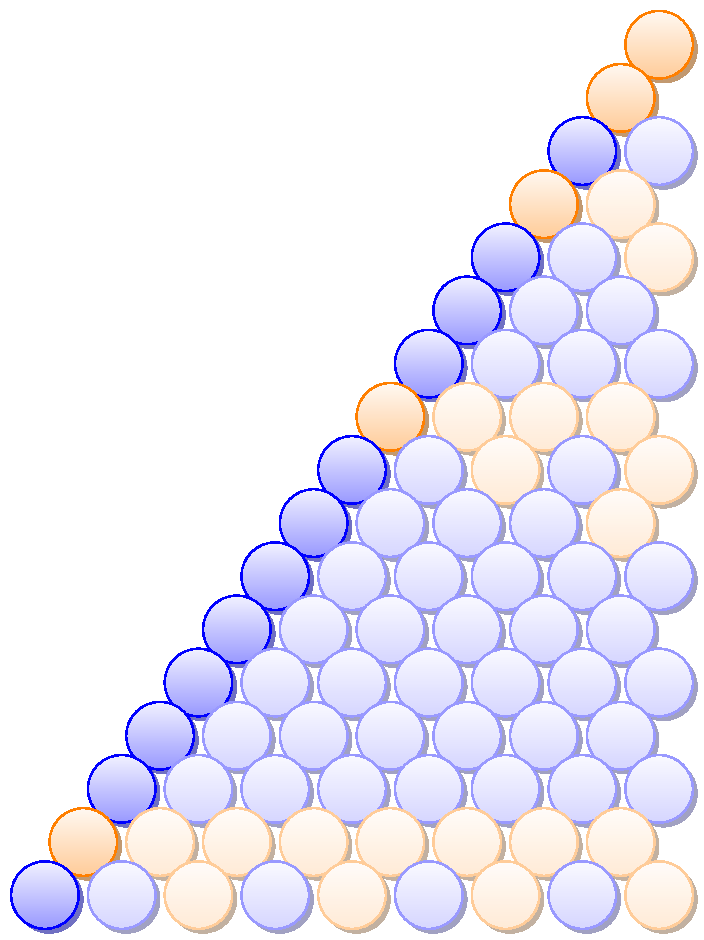
\includegraphics[
            width=7cm, 
            height=6cm, 
            keepaspectratio=true]{catalan-tikz/first-column/first-column.pdf}
    }

    % this 'particular' line is necessary to use `displaymath' environment
    % into the caption environment, togheter with the inclusion of 
    % `caption' package. See here for more explanation:
    % http://stackoverflow.com/questions/2716227/adding-an-equation-or-formula-to-a-figure-caption-in-latex
    \captionsetup{singlelinecheck=off}
    \caption[.]{ \textcolor{blue}{even},
        \textcolor{orange}{odd}  }

    \label{fig:catalan-first-column}

\end{figure}

        \end{column}
        \begin{column}[T]{5cm} % each column can also be its own environment
            let $d_{nk}\in\mathcal{C}$ and $c_{j}=d_{j0}$ be a Catalan number
            \begin{theorem}
                \begin{displaymath}
                    c_{j} \equiv_{2}1 \leftrightarrow j=2^{\alpha}-1
                \end{displaymath}
                where $\alpha\in\mathbb{N}$
            \end{theorem}
            \emph{proof}: $c_{j} = {{2j}\choose{j}} - {{2j}\choose{j+1}}$ and by cases on $j$'s parity
        \end{column}
    \end{columns}
\end{frame}

\begin{frame}{On $\mathcal{C}_{\equiv_{2}}$}
     $\mathcal{C}_{-(0,p^{h}-1)}^{h}$ be a copy of 
        $\mathcal{C}_{h}$:
        \begin{itemize}
            \item without $d_{nn}$ for each $n$ (antidiagonal $0$)
            \item without $d_{p^{h}-1,k}$ for each $k$ (row $p^{h}-1$)
        \end{itemize}
    \pause
    \begin{theorem}
        $h\in\mathbb{N}$ and $s\in\lbrace0,\ldots,2^{h}-1 \rbrace$, then 
            $d_{2^{h}-1,s} \equiv_{2} 1$
    \end{theorem}
    \emph{proof}: $ d_{2^{\alpha}-1,s} = \sum_{i_{1}+i_{2}+\ldots+i_{s+1}=2^{\alpha}}
                {c_{i_{1}-1}\,c_{i_{2}-1}\ldots\,c_{i_{s+1}-1}}$
    
\begin{figure}[p]

    \noindent\makebox[\textwidth]{
        \centering
        %\includegraphics[width=0.8\textwidth]{../../sympy/catalan/coloured.pdf}

        % using *angle* property to rotate it is difficult to properly align it
        % in order to have a "real" matrix representation.
        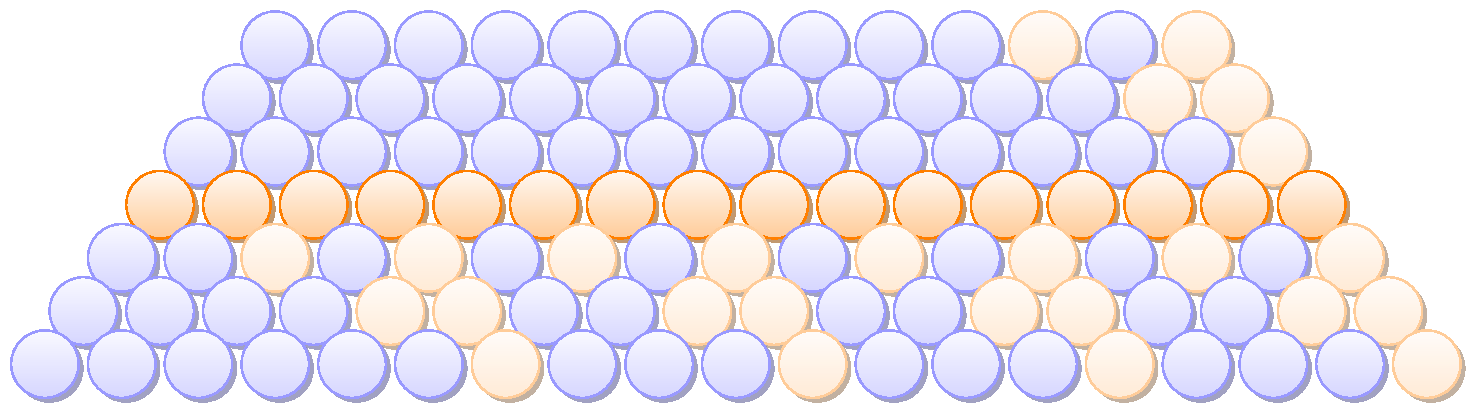
\includegraphics[width=10cm, height=10cm, keepaspectratio=true]
            {../RART2015/catalan-tikz/odd-row/odd-row.pdf}
    }

    % this 'particular' line is necessary to use `displaymath' environment
    % into the caption environment, togheter with the inclusion of 
    % `caption' package. See here for more explanation:
    % http://stackoverflow.com/questions/2716227/adding-an-equation-or-formula-to-a-figure-caption-in-latex
    \captionsetup{singlelinecheck=off}
    \caption[Row $\vect{r}_{2^{4}-1}$ of $\mathcal{C}_{\equiv_{2}}$]{
        Row $\vect{r}_{2^{4}-1}$ composed of coefficients $\textcolor{orange}{d_{2^{4}-1,s} \equiv_{2} 1}$, 
        for $s\in\lbrace1,\ldots,2^{4}-1 \rbrace$ }

    \label{fig:catalan-odd-row}

\end{figure}

\end{frame}

\begin{frame}{On $\mathcal{C}_{\equiv_{2}}$}
    \begin{theorem}
        let  $S=\lbrace2^{\alpha},\ldots,2^{\alpha+1}-2\rbrace$ be a segment of 
        column $2^{\alpha}-1$, then $d_{s,2^{\alpha}-1}\equiv_{2}0$ for $s\in S$
    \end{theorem}
    \emph{proof}: $d_{s, 2^{\alpha}-1} = \sum_{i_{1}+i_{2}+\ldots+i_{2^{\alpha}}=s+1}
            {c_{i_{1}-1}\,c_{i_{2}-1}\ldots\,c_{i_{2^{\alpha}}-1}}$
    
    
\begin{figure}[htb]

    \noindent\makebox[\textwidth]{
        \centering
        %\includegraphics[width=0.8\textwidth]{../../sympy/catalan/coloured.pdf}

        % using *angle* property to rotate it is difficult to properly align it
        % in order to have a "real" matrix representation.
        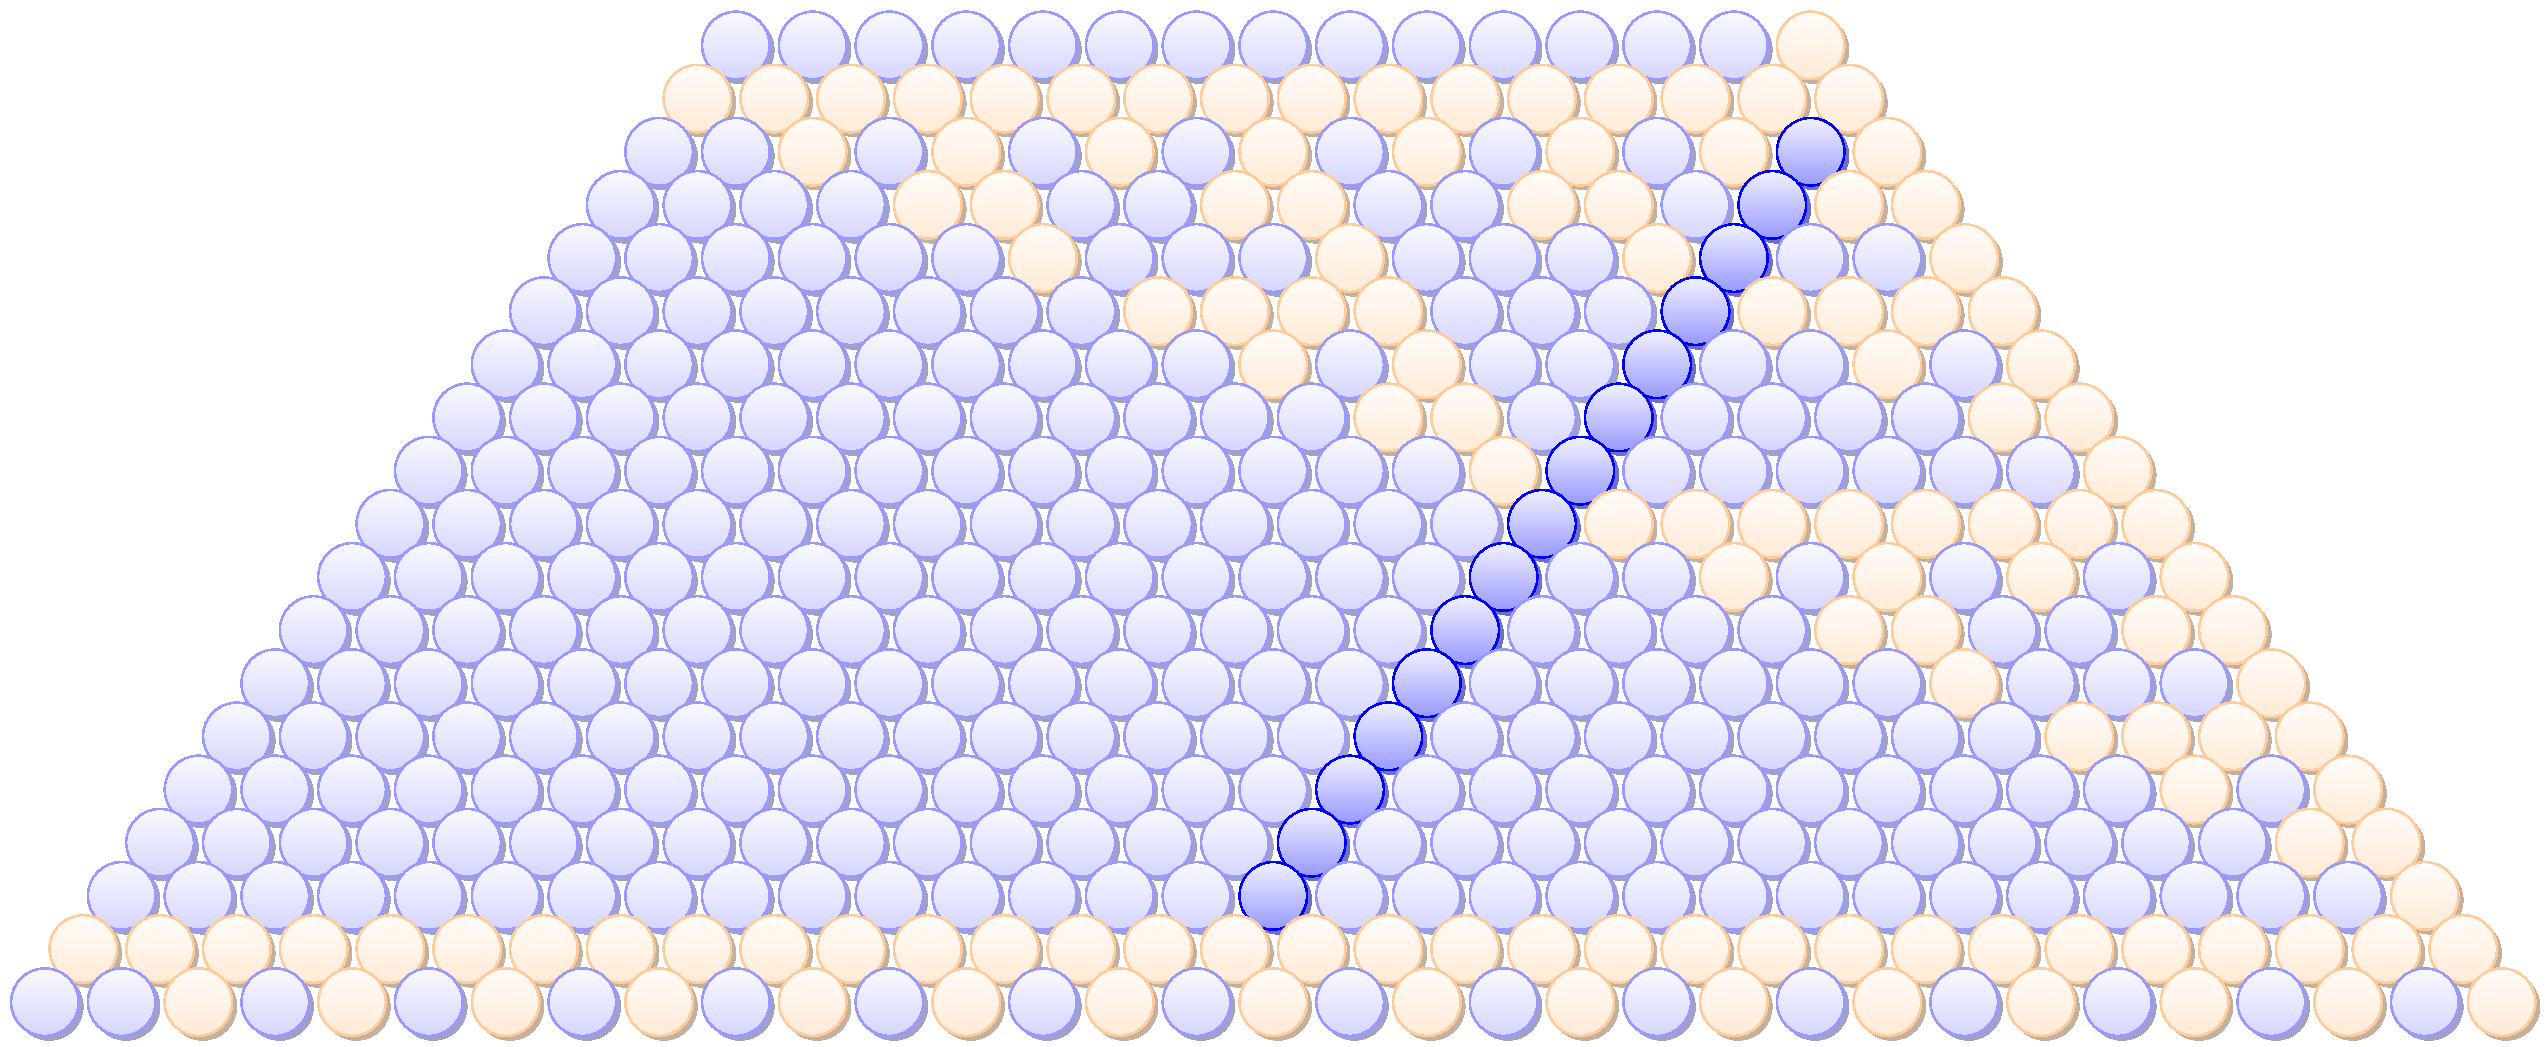
\includegraphics[width=10cm, height=10cm, keepaspectratio=true]
            {../RART2015/catalan-tikz/mirror-segment/mirror-segment.pdf}
    }

    % this 'particular' line is necessary to use `displaymath' environment
    % into the caption environment, togheter with the inclusion of 
    % `caption' package. See here for more explanation:
    % http://stackoverflow.com/questions/2716227/adding-an-equation-or-formula-to-a-figure-caption-in-latex
    \captionsetup{singlelinecheck=off}
    \caption[\emph{Mirror} segment $\Phi^{(4)}$ in $\mathcal{C}_{\equiv_{2}}^{(5)}$]
        {\emph{Mirror} segment $\Phi^{(4)}=\diagup_{\lbrace 1,2,\ldots,2^{4}-1\rbrace}^{2^{4}-1}$
        in $\mathcal{C}_{\equiv_{2}}^{(5)}$ }

    \label{fig:mirror-segment}

\end{figure}

        
\end{frame}

\begin{frame}{On $\mathcal{C}_{\equiv_{2}}$}
    \begin{theorem}
        let  $S=\lbrace2^{\alpha},\ldots,2^{\alpha+1}-2\rbrace$ be a segment of 
        column $2^{\alpha}-1$, then $d_{s,2^{\alpha}-1}\equiv_{2}0$ for $s\in S$
    \end{theorem}
    \emph{proof}: $d_{s, 2^{\alpha}-1} = \sum_{i_{1}+i_{2}+\ldots+i_{2^{\alpha}}=s+1}
            {c_{i_{1}-1}\,c_{i_{2}-1}\ldots\,c_{i_{2^{\alpha}}-1}}$
    \pause
    \begin{theorem}
    let $\hat{d}_{s,2^{h}-1}$ lying on column $2^{h}-1$ within segment 
    $S_{2^{h}-1}=\lbrace 2^{h}+1,\ldots,2^{h+1}-2 \rbrace$, then:
        $d_{s-e,2^{h}-1-e} \equiv_{2} d_{s,2^{h}-1+e}$ \\
    for $e\in\lbrace1,\ldots,s-(2^{h}-1)-1\rbrace=\lbrace1,\ldots,s-2^{h}\rbrace$,
    \end{theorem}
    \emph{proof}: $ d_{nk}\in\mathcal{C}\leftrightarrow{{2n-k}\choose{n-k}} - {{2n-k}\choose{n-k-1}}$ and \emph{Lucas theorem}
    \pause
    \begin{theorem}
    let $\hat{d}_{s,2^{h}-1}$ lying on column $2^{h}-1$ within segment 
    $S_{2^{h}-1}=\lbrace 2^{h}+1,\ldots,2^{h+1}-2 \rbrace$, then:
        $d_{s,2^{h}-1+e} \equiv_{2} d_{s-2^{h},e-1} $ \\
    for $e\in\lbrace1,\ldots,s-(2^{h}-1)-1\rbrace=\lbrace1,\ldots,s-2^{h}\rbrace$,
    \end{theorem}
    \emph{proof}: as before
        
\end{frame}



\section*{Summary}

\begin{frame}{Summary}

  % Keep the summary *very short*.
  \begin{itemize}
  \item
    The \alert{first main message} of your talk in one or two lines.
  \item
    The \alert{second main message} of your talk in one or two lines.
  \item
    Perhaps a \alert{third message}, but not more than that.
  \end{itemize}
  
  % The following outlook is optional.
  \vskip0pt plus.5fill
  \begin{itemize}
  \item
    Outlook
    \begin{itemize}
    \item
      Something you haven't solved.
    \item
      Something else you haven't solved.
    \end{itemize}
  \end{itemize}
\end{frame}



% All of the following is optional and typically not needed. 
\appendix
\section<presentation>*{\appendixname}
\subsection<presentation>*{For Further Reading}

\begin{frame}[allowframebreaks]
  \frametitle<presentation>{For Further Reading}
    
  \begin{thebibliography}{10}
    
  \beamertemplatebookbibitems
  % Start with overview books.

  \bibitem{Author1990}
    A.~Author.
    \newblock {\em Handbook of Everything}.
    \newblock Some Press, 1990.
    
  \beamertemplatearticlebibitems
  % Followed by interesting articles. Keep the list short. 

  \bibitem{Sved1998}
    Marta Sved.
    \newblock Divisibility - with visibility.
    \newblock {\em The Mathematical Intelligencer}, 10(2):56--64, 1998.

  \end{thebibliography}
\end{frame}

\end{document}


